\subsection{Klassifikation} \label{klassifikation-1}

Wie bereits in Kapitel \ref{grundlagen-klassifikation-0} beschrieben ist das Ziel der Klassifizierung ein Klassifizierungsmodell zu trainieren, das in der Lage ist, Objekte in den Daten in die entsprechende Klasse zuzuordnen. Die Klassen entsprechen hierbei den Emotionen, die erkannt werden sollen: Gl{\"u}ck, Langeweile, Frustation und andere (d.h. alle Emotionen, die nicht Gl{\"u}ck, Langeweile oder Furstation entsprechen). \\

Als erstes wird der Datensatz in ein Trainigs- und Testset  aufgeteilt. 
Es gibt keine festgelegten Regeln {\"u}ber die Proportionen der Sets. 
Im Allgemeinen wird das Trainingsset aber gr{\"o}{\ss}er als das Testset gew{\"a}hlt.
Da die Leistungen des Klassifikators jedoch stark von der gew{\"a}hlten Aufteilung abh{\"a}ngen, ist es wichtig, sicherzustellen, dass dieser Schritt richtig durchgef{\"u}hrt wird.
Bei einem Datensatz mit mehreren Probanden empfiehlt sich f{\"u}r die Aufteilung zwischen Trainings- und Testsets die Durchf{\"u}hrung einer Leave-One-Subjekt-Out-Cross-Validierung (LOSOCV).
Die Idee besteht darin, $N$ verschiedene Aufteilungen des Datensatzes vorzunehmen, wobei $N$ die Anzahl der Personen ist, die Daten f{\"u}r den Datensatz bereitgestellt haben. 
F{\"u}r jeden dieser Splits wird der Testset aus den Daten eines Probanden aufgebaut, w{\"a}hrend die Daten der anderen Probanden das Trainingsset bilden. 
Anschlie{\ss}end wird ein Klassifizierer erstellt und ausgewertet. Dies wird f{\"u}r alle Probanden wiederholt, d.h. $N$ mal.
Die so erhaltenen $N$-Bewertungskennzahlen (eine pro Proband) k{\"o}nnen dann gemittelt werden, um eine Gesamtbewertung des Modells zu erhalten.
Es ist wichtig zu beachten, dass der LOSOCV-Ansatz bei einer hohen Anzahl von Probanden sehr rechenintensiv sein kann. \\

\begin{figure}[h] \centering{
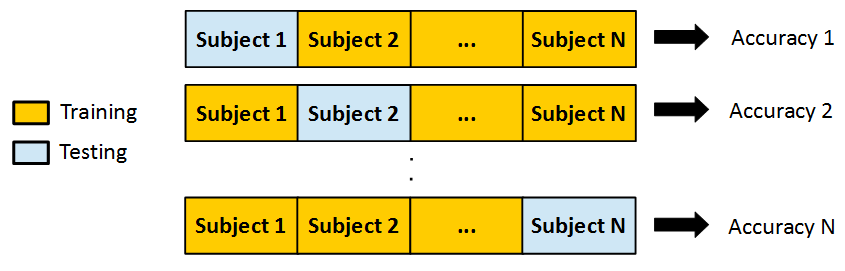
\includegraphics[width=15cm]{Images/LOSOCV.png} 
\caption[Leave-One-Subjekt-Out-Cross-Validation (LOSOCV)]{Leave-One-Subjekt-Out-Cross-Validation (LOSOCV): $N$ entspricht der Anzahl der Probanden. F{\"u}r jeden Split wird ein Testset aus den Daten eines Probanden aufgebaut, w{\"a}hrend die Daten der anderen Probanden einen Trainingsset bilden. Dieser Vorgang wird f{\"u}r die Daten jedes Probanden durchgef{\"u}hrt. }}
\label{fig:losocv} \end{figure} \vspace{0.5cm}